\section{Trajectory Planning - Laparoscopic tool manipulation}

At this step, given the points of the desired path, a more detailed trajectory is calculated, 
which will contain all the waypoints that the robot will have to visit. Trajectory planning is executed after a desired path is generated,
and consists in mapping the geometric points to specific \textbf{time points}, as well as assigning specific \textbf{velocities}, \textbf{accelerations} and \textbf{jerks}, 
in order to generate the commands needed for the robot controller to execute a smooth motion.\\

The paths that are calculated are parameterized by the path parameter $s$. As $s$ increases from $0$, the robot moves from the start configuration $q(0)$ to the goal configuration $q(1)$. 
Path planning outputs geometric information $q(s), s \in [0, 1]$, whereas the \textbf{trajectories} that are the subject of this chapter, also include \textbf{time information} $q(t), t \in [0, T]$. 
A path can be converted to a trajectory by defining a function $s(t): [0, T] \rightarrow [0, 1]$ which maps the time parameter's range to the path parameter's range. This function is also known as \textbf{time scaling} or 
\textbf{time parameterization}.The most common methodology of trajectory planning, which is also used in this thesis, is the one that is studied in the \textbf{joint angles space} also known as \textbf{configuration space}.\\

The biggest challenge in manipulating a laparoscopic tool with a robot is overcoming the \textbf{fulcrum effect} problem. This is also one of the reasons that 
robotic assisted surgery replaced the traditional laparoscopic procedures. The fulcrum effect means that the surgeon's hand motions are inverted and scaled 
with respect to the Remote Center of Motion point, which lies approximately on the center of the incision. Apart from the scaling and inversion, laparoscopic 
procedures add an additional motion constraint that demands at each time one point of the laparoscopic tool to coincide with the RCM point.\\

\subsection{Tool pose \& the Fulcrum Effect}

\begin{center}
\begin{figure}[H]
\centering
\includegraphics[width=12cm]{images/fulcrum-space.png}\\
\caption{Tool pose at target point $B$ calculated with respect to Fulcrum's reference frame $\lbrace F \rbrace$}
\end{figure}
\end{center}

The laparoscopic tool pose is given by the position and orientation vectors at target point $B$ with respect to the coordinate frame $\lbrace F \rbrace$.
The pose is given by the following transformation matrix
\[
{}^{F}T_B = \begin{bmatrix}
{}^{F}R_B & {}^{F}\mathbf{p}^{}_B \\
\mathbf{0} & 1 \\
\end{bmatrix}
\;\; where \;\;
{}^{F}R_B = \begin{bmatrix}
\hat{\mathbf{x}}^{}_B & \hat{\mathbf{y}}^{}_B & \hat{\mathbf{z}}^{}_B \\
\end{bmatrix}
\]

\begin{equation}
\hat{\mathbf{x}}^{}_B = \hat{\mathbf{θ}} = cos(θ)cos(φ)\hat{\mathbf{x}}^{}_F + cos(θ)sin(φ)\hat{\mathbf{y}}^{}_F - sin(θ)\hat{\mathbf{z}}^{}_F
= \begin{bmatrix}
cos(θ)cos(φ) \\
cos(θ)sin(φ) \\
- sin(θ) \\
\end{bmatrix}
\end{equation}

\begin{equation}
\hat{\mathbf{y}}^{}_B = \hat{\mathbf{φ}} = -sin(φ)\hat{\mathbf{x}}^{}_F + cos(φ)\hat{\mathbf{y}}^{}_F
= \begin{bmatrix}
-sin(φ) \\
cos(φ) \\
0 \\
\end{bmatrix}
\end{equation}

\begin{equation}
\hat{\mathbf{z}}^{}_B = - \hat{\mathbf{r}} = - (sin(θ)cos(φ)\hat{\mathbf{x}}^{}_F + sin(θ)sin(φ)\hat{\mathbf{y}}^{}_F + cos(θ)\hat{\mathbf{z}}^{}_F)
= \begin{bmatrix}
-sin(θ)cos(φ) \\
-sin(θ)sin(φ) \\
-cos(θ) \\
\end{bmatrix}
\end{equation}

The position of the point $B$ is given in spherical coordinates by:
\begin{itemize}
	\item $r=ρ$ : outside penetration of laparoscopic tool
	\item $θ=β$ : altitude angle
	\item $φ=α$ : orientation angle
\end{itemize}
thus the position with respect to the coordinate frame $\lbrace F \rbrace$ is given by
\begin{equation}
{}^{F}\mathbf{p}^{}_B = \begin{bmatrix}
ρsin(β)cos(α) \\
ρsin(β)sin(α) \\
ρcos(β) \\
\end{bmatrix} = ρ \hat{\mathbf{r}}
\end{equation}

The above goal point must be the same as the $TCP$ point of the robot's end-effector. This means, that this pose must be converted with respect to the robot's reference frames.
\[
{}^{U}T^{}_{TCP} = {}^{U}T^{}_{B}
\]
\[
{}^{U}T^{}_{0} \; {}^{0}T^{}_{7} \; {}^{7}T^{}_{TCP} = {}^{U}T^{}_{F} \; {}^{F}T^{}_{B}
\]
\begin{equation}
{}^{0}T^{}_{7} = {}^{U}T^{-1}_{0} \; {}^{U}T^{}_{F} \; {}^{F}T^{}_{B} \; {}^{7}T^{-1}_{TCP}
\end{equation}

\begin{listing}[H]
\begin{minted}[tabsize=2,breaklines,frame=lines,framesep=2mm,baselinestretch=1.2,fontsize=\footnotesize, linenos]{matlab}
function tcp = fulcrumEffectTrajectory(P, L)
    tcp = zeros(size(P));
    for i=1:size(P)
        px = P(i,1); py = P(i,2); pz = P(i,3);
        r = sqrt(px^2+py^2+pz^2);
        th = atan2(sqrt(px^2+py^2), pz);
        phi = atan2(py, px);
        vx = [cos(th)*cos(phi); cos(th)*sin(phi); -sin(th)];
        vy = [-sin(phi); cos(phi); 0];
        vz = [-sin(th)*cos(phi); -sin(th)*sin(phi); cos(th)];
        vp = r*[sin(th)*cos(phi); sin(th)*sin(phi); cos(th)];
        T = zeros(4,4);
        R = [vx, vy, vz];
        T(1:3,1:3) = R;
        T(1:3,4) = vp;
        T(4,4) = 1;
        Td = eye(4);
        Td(1:3,4) = (r-L)/r*vp;
        tcp_point = Td*inv(T)*[P(i,:).'; 1];
        tcp(i,:) = tcp_point(1:3).';
    end
end
\end{minted}
\caption{Fulcrum Effect transformation of a trajectory, in MATLAB}
\label{code:fulcrum_effect_traj_matlab}
\end{listing}


\subsection{Trajectory planning in cartesian coordinates}
\label{subsection:pivot-motions}

On this section, some basic pivoting trajectories around the fulcrum point, are presented. In all of the following three example pivoting motions, we have made 
the assumption that the position and orientation of the ${F}$ reference frame is precisely known, which is however not applicable in real-life scenarios. The trajectories 
presented in this section are planned in cartesian coordinates or also known as \textbf{Task space}.

\underline{Advantages of planning in Task Space}
\begin{itemize}
\item Since the interpolation of the path points is in task space, then the planned motion is \textbf{more predictable}.
\item It is easier to design trajectories which are \textbf{better in avoiding obstacles and handling collisions}.
\end{itemize}

\underline{Disadvantages of planning in Task Space}
\begin{itemize}
\item \textbf{Planning and execution are significantly slower}, because for each interpolation point in task space the Inverse Kinematics problem must be solved. This issue is
even more problematic when the IK problem is not solved with analytical equations but numerically using optimization techniques.
\item A smooth trajectory in task space is not necessarily smooth in Joint Space.
\end{itemize}

\subsubsection{Circular trajectory of tool tip}

\begin{center}
\begin{figure}[H]
\centering
\includegraphics[width=0.8\textwidth]{images/circular-trajectory-wrt-fulcrum.png}\\
\caption{Circular trajectory of tool tip with respect to Fulcrum reference frame}
\end{figure}
\end{center}

To generate a circular trajectory for the pivot movement we must specify the center of the circle 
and a vector whose magnitude is the radius of the circle and it’s direction gives the orientation 
of the plane that the circle lies at. The simplest case of a circular trajectory is the one, 
whose circle lies in a plane parallel to the xy plane.


We first consider the motion of the laparoscopic tool tip on a circle parallel to a z-plane, with respect to the $\lbrace F \rbrace$ coordinate frame.
\begin{equation}
(x^{}_{F} - x^{}_{F0})^2 + (y^{}_{F} - y^{}_{F0})^2 = r_0^2, \;\; z^{}_{F} = z^{}_{F0}
\end{equation}
It's often more convenient to express trajectories in a parametric form, which makes it easier to calculate all the waypoints of the trajectory
\begin{equation}
\begin{cases}
x^{}_{F} = r_0cos(2πs) + x^{}_{F0} \\
y^{}_{F} = r_0sin(2πs) + y^{}_{F0} \\
z^{}_{F} = z^{}_{F0}
\end{cases} ,
\;\;
s \in [0, 1]
\end{equation}

After having calculated the cartesian coordinates we can calculate the spherical coordinates as follows

\begin{equation}
\label{eqns:cartesian-to-spherical}
\begin{cases}
r = \sqrt{x^{2}_{F} + y^{2}_{F} + z^{2}_{F}} \\
θ = atan2 \left( \sqrt{x^{2}_{F} + y^{2}_{F}}, z^{}_{F} \right) \\
φ = atan2(y^{}_{F}, x^{}_{F})
\end{cases}
\end{equation}

\begin{center}
\begin{figure}[H]
\centering
\includegraphics[width=\textwidth]{images/rcm_trajectories/rcm_circle_traj.png}\\
\caption{Circular trajectory of tool tip with respect to Fulcrum reference frame and it's transformation via the Fulcrum Effect}
\end{figure}
\end{center}


\subsubsection{Circular arc trajectory of tool tip}

To generate a circular arc trajectory for a pivot motion we must specify the same parameters as 
in the circular trajectory as well as the length of the arc or the total angle $φ$ of the arc 
section. Another parameter has more significance in circular arc trajectories that plain circles is the phase of the arc. This initial phase can be expressed as either an angle $φ_0$ added to the arguments of 
sine and cosine functions or it can be expressed as $s$ values that have as initial value different from $0$. The parametric equations for a circular arc are:

\begin{equation}
\begin{cases}
x^{}_{F} = r_0cos(2πs + φ_0) + x^{}_{F0} \\
y^{}_{F} = r_0sin(2πs + φ_0) + y^{}_{F0} \\
z^{}_{F} = z^{}_{F0}
\end{cases} ,
\;\;
s \in \left[ 0, \frac{φ}{2π} \right]
\end{equation}

\begin{center}
\begin{figure}[H]
\centering
\includegraphics[width=\textwidth]{images/rcm_trajectories/rcm_arcs_traj.png}\\
\caption{Circular arc trajectory of tool tip with respect to Fulcrum reference frame and it's transformation via the Fulcrum Effect. In this trajectory 2 circular arcs are used}
\end{figure}
\end{center}

\subsubsection{Line segment trajectory of tool tip}

\begin{center}
\begin{figure}[H]
\centering
\includegraphics[width=10cm]{images/line-segment-trajectory-wrt-fulcrum.png}\\
\caption{Line segment trajectory of tool tip with respect to Fulcrum reference frame}
\end{figure}
\end{center}
\[
\mathbf{d} = {}^{F}\mathbf{p}^{}_{T2} - {}^{F}\mathbf{p}^{}_{T1} = [l, m, n]^\top
\]
\[
{}^{F}\mathbf{p}^{}_{T} = [x^{}_{F}, y^{}_{F}, z^{}_{F}]^\top
\]
\[
{}^{F}\mathbf{p}^{}_{T} = {}^{F}\mathbf{p}^{}_{T1} + s\mathbf{d}
\]
\[
s = \frac{x^{}_{F} - x^{}_{F1}}{l} = \frac{y^{}_{F} - y^{}_{F1}}{m} = \frac{z^{}_{F} - z^{}_{F1}}{n} \;\; s \in [0, 1]
\]

\begin{equation}
\begin{cases}
x^{}_{F} = sl + x^{}_{F1} = (1-s)x^{}_{F1} + sx^{}_{F2} \\
y^{}_{F} = sm + y^{}_{F1} = (1-s)y^{}_{F1} + sy^{}_{F2} \\
z^{}_{F} = sn + z^{}_{F1} = (1-s)z^{}_{F1} + sz^{}_{F2}
\end{cases}
\end{equation}

After having calculated the cartesian coordinates we can calculate the spherical coordinates using the \ref{eqns:cartesian-to-spherical} equations.

\begin{center}
\begin{figure}[H]
\centering
\includegraphics[width=\textwidth]{images/rcm_trajectories/rcm_lineseg_traj.png}\\
\caption{A Line segment trajectory and it's transformation via the Fulcrum Effect}
\end{figure}
\end{center}

The line segment trajectory of tool tip, as analysed above, \textbf{should not be confused with the} computeCartesianPath method provided by ROS MoveIt library that can be used to create line segment 
trajectories. This method produces line segment trajectories for the end effector of the robot which are not transformed as line segments via the Fulcrum Effect.

\subsubsection{Cubic Spline trajectory of tool tip}

A useful mathematical tool to construct a smooth curve that visits every point from a given set of waypoints are \textbf{cubic splines}. A cubic spline is 
constructed using smaller curves that are described by a polynomial of 3rd order. Let $\left\lbrace \mathbf{P}_0, \mathbf{P}_1, \ldots , \mathbf{P}_n \right\rbrace$ 
be a set of waypoints, where each point has coordinates $\mathbf{P}_i = [x_i, y_i, z_i]^\top$. Then between each 2 points a cubic 
polynomial can be constructed (one for each coordinate, 3 in total). The following equations are for the $x$-coordinate and in the exact same way one can 
calculate the cubic polynomials for the $y,z$ coordinates as well. For each pair of waypoints we want to calculate the following cubic polynomial
\begin{equation}
\label{cubic-polynomial}
x_i(s) = a_i(s-s_i)^3 + b_i(s-s_i)^2 + c_i(s-s_i) + d_i, \hspace{3em} s_i \leqslant s \leqslant s_{i+1}
\end{equation}

The polynomial in equation \ref{cubic-polynomial} has four unknowns which means that four additional equations are needed to get a unique solution and fully 
define the polynomial. These equations can be formed using the boundary conditions for the first and last point of each curve.
\begin{equation}
x_i(s_i) = x_i
\end{equation}
\begin{equation}
x_i(s_{i+1}) = x_{i+1}
\end{equation}
\begin{equation}
\dot{x}_i(s_i) = \dot{x}_i
\end{equation}
\begin{equation}
\dot{x}_i(s_{i+1}) = \dot{x}_{i+1}
\end{equation}

First we solve for $c_i$ and $d_i$, which can easily be calculated as follows
\begin{equation}
\label{di-eq}
d_i = x_i(s_i) = x_i
\end{equation}
and by taking the derivative of \ref{cubic-polynomial}, we can calculate $c_i$
\begin{equation}
\label{cubic-polynomial-first-derivative}
\dot{x}_i(s_i) = 3a_i(s-s_i)^2 + 2b_i(s-s_i) + c_i
\end{equation}
\begin{equation}
\label{ci-eq}
c_i = \dot{x}_i(s_i) = \dot{x}_i
\end{equation}

By substituting $s = s_{i+1}$ in \ref{cubic-polynomial} and \ref{cubic-polynomial-first-derivative}, by using equations \ref{ci-eq}, \ref{di-eq} and if 
we set $σ = s_{i+1}-s_i$ for brevity, we get the following two equations
\begin{equation}
\label{xi1}
x_{i+1} = x_i(s_{i+1}) = a_i σ^3 + b_i σ^2 + c_i σ + x_i
\end{equation}
and
\begin{equation}
\label{xdi1}
\dot{x}_{i+1} = \dot{x}_i(s_{i+1}) = 3a_i σ^2 + 2b_i σ + \dot{x}_i
\end{equation}

By multiplying \ref{xdi1} by $σ$ and \ref{xi1} by $-3$ and add them together we get
\[
\dot{x}_{i+1}σ - 3x_{i+1} = -b_iσ^2 -2\dot{x}_iσ - 3x_i
\]
\begin{equation}
b_i = \frac{1}{σ^2} (3x_{i+1} -3x_i - \dot{x}_{i+1}σ - 2\dot{x}_iσ)
\end{equation}

Similarly, by multiplying \ref{xdi1} by $σ$ and \ref{xi1} by $-2$ and add them together we get
\[
\dot{x}_{i+1}σ - 2x_{i+1} = a_iσ^3 -\dot{x}_iσ - 2x_i
\]
\begin{equation}
a_i = \frac{1}{σ^3} (\dot{x}_{i+1}σ - 2x_{i+1} + \dot{x}_iσ +2x_i)
\end{equation}

\begin{center}
\begin{figure}[H]
\centering
\includegraphics[width=\textwidth]{images/cubic-spline-path1.png}\\
\caption{Cubic Spline curve with 10 waypoints} 
\label{cubic-spline-explanation}
\end{figure}
\end{center}

\begin{center}
\begin{figure}[H]
\centering
\includegraphics[width=\textwidth]{images/rcm_trajectories/rcm_cubic_traj.png}\\
\caption{A Cubic Spline trajectory and it's transformation via the Fulcrum Effect}
\end{figure}
\end{center}


\subsubsection{B-Spline trajectory of tool tip}

The \textbf{B-Splines} are smooth curves which are constructed from \textbf{B\'ezier} curves. A B\'ezier curve is a parametric smooth curve and is a $k$-th order interpolation of $k+1$ control points.

\begin{center}
\begin{figure}[H]
\centering
\includegraphics[width=0.5\textwidth]{images/bezier-curve.png}\\
\caption{Cubic B\'ezier curve calculated using cubic interpolation of 4 control points} 
\end{figure}
\end{center}

We first calculate the linear interpolation of the control points
\begin{equation}
\mathbf{L}_0(s) = (1-s)\mathbf{P}_0 + s\mathbf{P}_1
\end{equation}
\[
\mathbf{L}_1(s) = (1-s)\mathbf{P}_1 + s\mathbf{P}_2
\]
\[
\mathbf{L}_2(s) = (1-s)\mathbf{P}_2 + s\mathbf{P}_3
\]
The next step is to calculate the quadratic interpolation of the control points or equivalently, the linear interpolation of the previously calculated points $\mathbf{L}_0,\mathbf{L}_1,\mathbf{L}_2$
\[
\mathbf{Q}_0(s) = (1-s)\mathbf{L}_0(s) + s\mathbf{L}_1(s)
\]
\begin{equation}
\mathbf{Q}_0(s) = (1-s)^2\mathbf{P}_0 + 2(1-s)s\mathbf{P}_1 + s^2\mathbf{P}_2
\end{equation}
\[
\mathbf{Q}_1(s) = (1-s)^2\mathbf{P}_1 + 2(1-s)s\mathbf{P}_2 + s^2\mathbf{P}_3
\]
Similarly for the last step, we calculate the cubic interpolation of the control points or equivalently, the linear interpolation of the previously calculated points $\mathbf{Q}_0,\mathbf{Q}_1$
\[
\mathbf{C}_0(s) = (1-s)\mathbf{Q}_0(s) + s\mathbf{Q}_1(s)
\]
\begin{equation}
\mathbf{C}_0(s) = (1-s)^3\mathbf{P}_0 +3(1-s)^2 s\mathbf{P}_1 + 3(1-s)s^2\mathbf{P}_2 + s^3\mathbf{P}_3
\end{equation}

The cubic B\'ezier curve can also be calculated using the following more compact equation, in matrix form
\begin{equation}
\mathbf{C}_0(s) = \begin{bmatrix} \mathbf{P}_0 & \mathbf{P}_1 & \mathbf{P}_2 & \mathbf{P}_3 \end{bmatrix} 
\begin{bmatrix} 
-1 & 3 & -3 & 1 \\
3 & -6 & 3 & 0 \\
-3 & 3 & 0 & 0 \\
1 & 0 & 0 & 0
\end{bmatrix}
\begin{bmatrix}
s^3 \\ s^2 \\ s \\ 1
\end{bmatrix}
\end{equation}

\begin{center}
\begin{figure}[H]
\centering
\includegraphics[width=\textwidth]{images/bezier_path.png}\\
\caption{A cubic B\'ezier curve calculated and plotted in MATLAB} 
\end{figure}
\end{center}

A $k$-degree \textbf{B-Spline} curve defined by $n+1$ control points will consist of $n-k+1$ B\'ezier curves. For example if we want to construct a cubic B-Spline using 6 control points, then we will need to construct 
and connect together 3 B\'ezier curves.

\begin{center}
\begin{figure}[H]
\centering
\includegraphics[width=0.6\textwidth]{images/b-spline-explanation.png}\\
\caption{B-Spline curve constructed from 3 B\'ezier curves. The first B\'ezier curve colored in red is a quadratic one and the following two are both cubic.} 
\label{b-spline-explanation}
\end{figure}
\end{center}

In most cases the B-Spline curves are constructed by starting from a quadratic B\'ezier curve, which is constructed from 3 control points and then all other 
parts of the curve are constructed from cubic B\'ezier curves, each constructed from 4 control points. As shown in figure \ref{b-spline-explanation}, the B-Spline 
curves do not pass from all control points. This means that if we have a path formed by a set of waypoints and we want the robot to pass from all of them, then 
in order to construct a B-Spline trajectory we will need additional intermediary points. The first and last points are part of the curve and the other control 
points are not. If no additional points can be calculated then the robot will not pass from all the points, which in some cases is also acceptable and useful. \\

One must notice also, in figure \ref{b-spline-explanation} for example, that some points must be colinear in order for the transition from one B\'ezier curve to another to be smooth, or equivalently 
the point where the two curves are connected to have a continuous derivative. For example in figure \ref{b-spline-explanation}, $\mathbf{P}_2, \mathbf{P}_3, \mathbf{P}_4$ must be colinear so that the 
derivative of the curve at $\mathbf{P}_3$ is continuous. In the same example one can also notice that if the distance of $\overrightarrow{\mathbf{P}_2\mathbf{P}_3}$ and $\overrightarrow{\mathbf{P}_3\mathbf{P}_4}$ 
is getting smaller then the curve at $\mathbf{P}_3$ is getting sharper and if these distances are $0$ then instead of a smooth curve we have a sharp corner and the curve has 
no longer a continuous derivative at $\mathbf{P}_3$. These two parameters; \textbf{3 colinear points} and the \textbf{distances of the two vectors} of these 3 colinear points can be very useful in designing 
B-Spline trajectories when we only have the waypoints available and not the extra control points required to construct the B\'ezier curves.\\

It is very important that the designed trajectory respects the joints angles' range. For example
depending on the starting position of the circular trajectory depicted at figure 
\ref{fig:circ-traj-out-of-angle-range}, the robot arm may reach it's joint bounds and in order to 
continue executing the trajectory it will have to make a sudden jump to reset the angles. 
This could have serious side-effects for both the surgical task and thus the patient, as well as 
for the operating staff, who control the robot.

\begin{center}
\begin{figure}[H]
\centering
\includegraphics[width=\textwidth]{images/rcm_trajectories/rcm_bezier_traj.png}\\
\caption{A B\'ezier curve trajectory and it's transformation via the Fulcrum Effect}
\end{figure}
\end{center}


\subsection{Trajectory planning in joint angles space}

\underline{Advantages of planning in Joint Space}
\begin{itemize}
\item Planning trajectories in Joint Space is \textbf{much faster in execution} than Task Space planning, because the Inverse Kinematics problem is solved for fewer points, only at the waypoints of the trajectory 
and not at the intermediate points (the points between the waypoints).
\item The actuators' motion is smoother
\end{itemize}

\underline{Disadvantages of planning in Joint Space}
\begin{itemize}
\item The interpolated intermediate points are not guaranteed to be collision-free.
\end{itemize}

\begin{center}
\begin{figure}[H]
\centering
\includegraphics[width=\textwidth]{images/trajectory1-test1.png}\\
\caption{Trajectory diagrams in joints space.}
\end{figure}
\end{center}


\subsubsection{Polynomials of 5th order}


\subsubsection{Trapezoidal velocity profile}


\subsubsection{S-Curve velocity profile}